\subsection{Comparison of Accuracy vs Order}

It would be interesting to investigate whether the accuracy changes depending on
the transfer function's order $n$.

For each  order $n$ 100 random PTn transfer functions $G_n(s)$ were generated in
the form of:

\begin{equation}
    G(s) = \prod_{k=1}^n \frac{1}{s+T_k}
    \label{eq:random_ptn}
\end{equation}

where $n$ was a random integer in  the  range of $[2..8]$ and $T_k$ was a random
number in the range of $[1..9]$.

The step response of each $G_n(s)$  was fed into each method. The step responses
of each resulting transfer  function  was  then  compared  to the original input
function's step  response  and the root mean square error (RMSE) was calculated.
The  100 errors were then averaged, resulting in a final error  value  for  each
method, for each order.

\begin{figure}
    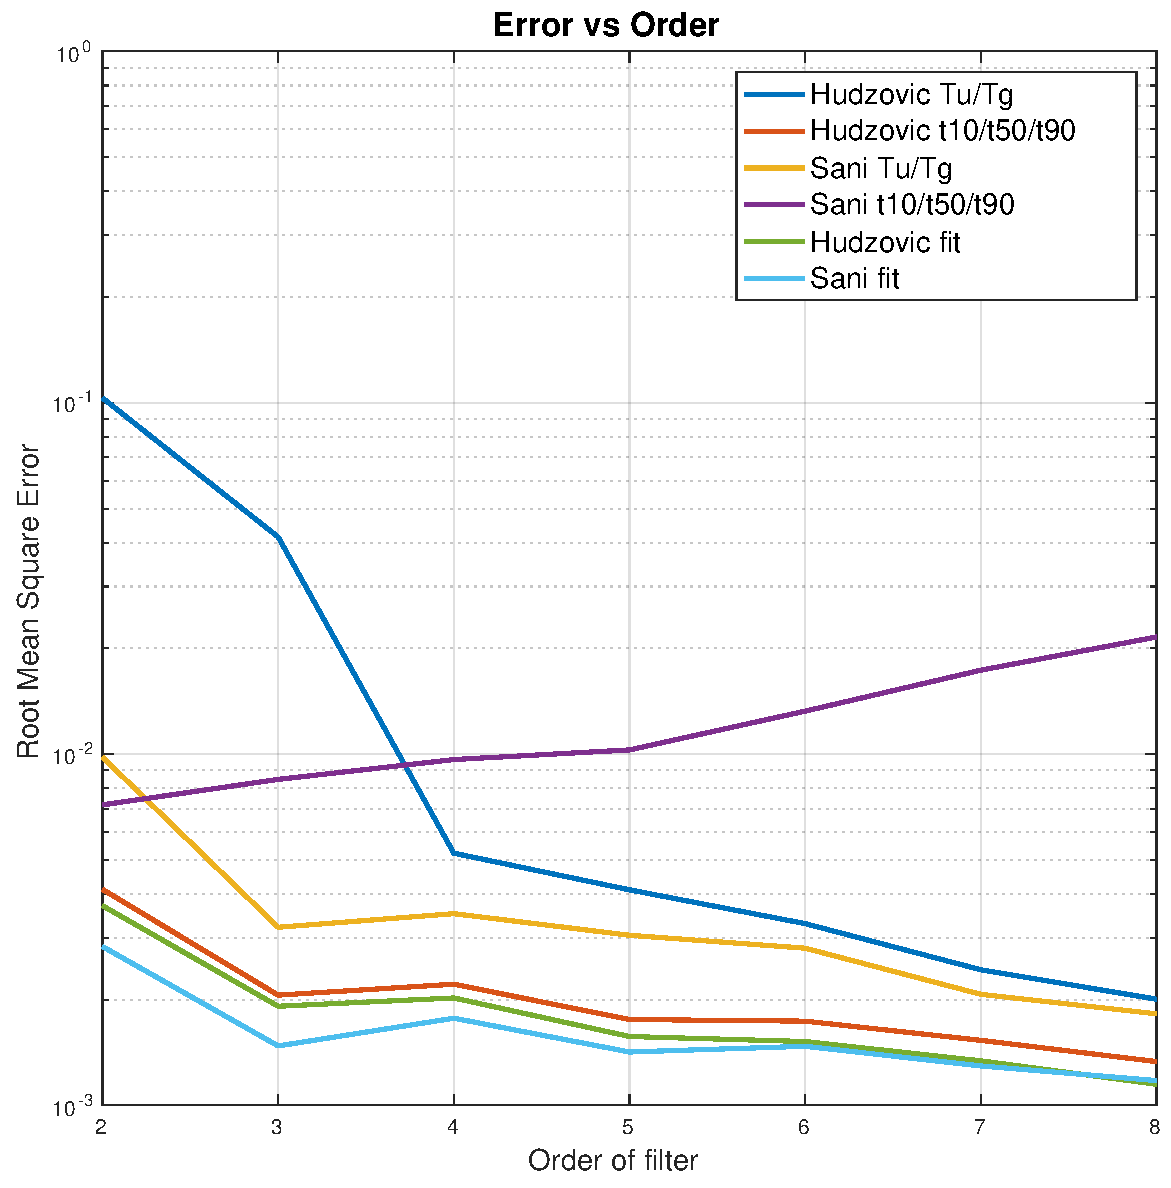
\includegraphics[width=\linewidth]{images/error_order}
    \caption{The mean square error (MSE) of each method to a randomly generated step response, in function of filter order}
    \label{fig:error_order}
\end{figure}
\begin{figure}
    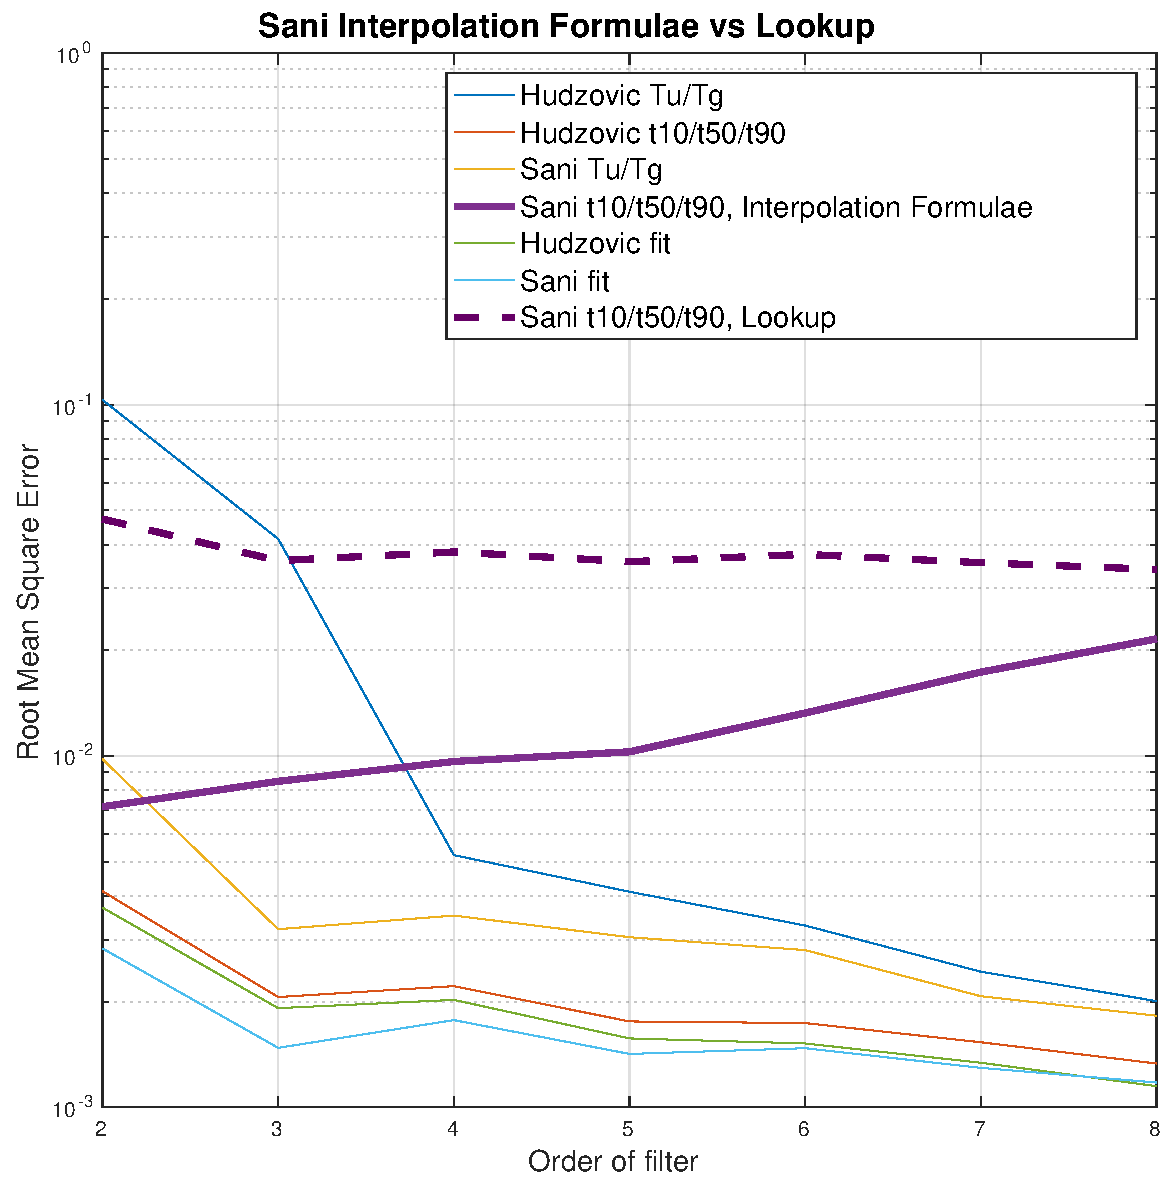
\includegraphics[width=\linewidth]{images/sani_interpolation_vs_lookup}
    \caption{Interpolation formulae proposed by L. Sani compared to ``brute force'' calculating the individual t10, t50, t90 parameters and creating lookup curves}
    \label{fig:interpolation_vs_lookup}
\end{figure}

The data portrayed in figure \ref{fig:error_order} shows these errors.

\subsubsection*{Conclusions}

As expected, the fitted methods yield  the  most  accurate results. The Sani fit
appears to be better than the Hudzovic fit.

The  most  accurate  non-fitted  method  is  Hudzovic's   transfer  function  in
combination with Sani's characterisation (orange curve).

An interesting observation is that the method proposed by L. Sani\cite{ref:sani}
using the $t_{10}$, $t_{50}$,  $t_{90}$ characterisation (purple curve) performs
worse and worse the higher the order, whereas all  other  methods perform better
and  better.  The exact reason as to why this happens is a consequence of  using
the    interpolation     formulae     proposed     by    L.    Sani    (equation
\ref{eq:sani_interpolation}) rather than using lookup curves.

To  see  if  this  is indeed the cause, the MATLAB code was adapted such that L.
Sani's  method  for determining $r$, $T$, $n$ based on the input data  $t_{10}$,
$t_{50}$, $t_{90}$ used  a  lookup  curve  instead  of  using  the interpolation
formulae. The same simulation was performed again with the modified code.

The result can be seen in figure \ref{fig:interpolation_vs_lookup}.  The  purple
line is the same  purple  curve  from  figure  \ref{fig:error_order}. The dashed
purple line shows the result of the modification.

It appears that by using lookup curves the resulting  transfer  function is less
accurate than if interpolation formulae were used.

